%%%%%%%%%%%%%%%%%%%%%%%%%%%%%%%%%%%%%%%%%
% Beamer Presentation
% LaTeX Template
% Version 1.0 (10/11/12)
%
% This template has been downloaded from:
% http://www.LaTeXTemplates.com
%
% License:
% CC BY-NC-SA 3.0 (http://creativecommons.org/licenses/by-nc-sa/3.0/)
%
%%%%%%%%%%%%%%%%%%%%%%%%%%%%%%%%%%%%%%%%%

%----------------------------------------------------------------------------------------
%	PACKAGES AND THEMES
%----------------------------------------------------------------------------------------

\documentclass{beamer}

\usepackage{xcolor}
\usepackage{soul}

\mode<presentation> {

% The Beamer class comes with a number of default slide themes
% which change the colors and layouts of slides. Below this is a list
% of all the themes, uncomment each in turn to see what they look like.

%\usetheme{default}
%\usetheme{AnnArbor}
%\usetheme{Antibes}
%\usetheme{Bergen}
%\usetheme{Berkeley}
%\usetheme{Berlin}
%\usetheme{Boadilla}
%\usetheme{CambridgeUS}
%\usetheme{Copenhagen}
%\usetheme{Darmstadt}
%\usetheme{Dresden}
%\usetheme{Frankfurt}
%\usetheme{Goettingen}
%\usetheme{Hannover}
%\usetheme{Ilmenau}
%\usetheme{JuanLesPins}
%\usetheme{Luebeck}
\usetheme{Madrid}
%\usetheme{Malmoe}
%\usetheme{Marburg}
%\usetheme{Montpellier}
%\usetheme{PaloAlto}
%\usetheme{Pittsburgh}
%\usetheme{Rochester}
%\usetheme{Singapore}
%\usetheme{Szeged}
%\usetheme{Warsaw}

% As well as themes, the Beamer class has a number of color themes
% for any slide theme. Uncomment each of these in turn to see how it
% changes the colors of your current slide theme.

%\usecolortheme{albatross}
%\usecolortheme{beaver}
%\usecolortheme{beetle}
%\usecolortheme{crane}
%\usecolortheme{dolphin}
%\usecolortheme{dove}
%\usecolortheme{fly}
%\usecolortheme{lily}
%\usecolortheme{orchid}
%\usecolortheme{rose}
%\usecolortheme{seagull}
%\usecolortheme{seahorse}
%\usecolortheme{whale}
%\usecolortheme{wolverine}

%\setbeamertemplate{footline} % To remove the footer line in all slides uncomment this line
%\setbeamertemplate{footline}[page number] % To replace the footer line in all slides with a simple slide count uncomment this line

%\setbeamertemplate{navigation symbols}{} % To remove the navigation symbols from the bottom of all slides uncomment this line
}

\usepackage{graphicx} % Allows including images
\usepackage{booktabs} % Allows the use of \toprule, \midrule and \bottomrule in tables

%----------------------------------------------------------------------------------------
%	TITLE PAGE
%----------------------------------------------------------------------------------------

\title[AI System definitions]{An analysis on the definitions of “AI System”} % The short title appears at the bottom of every slide, the full title is only on the title page

\author{Alessandro Lorenzi, Luca Cazzola} % Your name
\institute[UNITN] % Your institution as it will appear on the bottom of every slide, may be shorthand to save space
{
University of Trento \\ % Your institution for the title page
\medskip
% \textit{john@smith.com} % Your email address
}
\date{\today} % Date, can be changed to a custom date

\begin{document}

\begin{frame}
\titlepage % Print the title page as the first slide
\end{frame}

% \begin{frame}
% \frametitle{Overview} % Table of contents slide, comment this block out to remove it
% \tableofcontents % Throughout your presentation, if you choose to use \section{} and \subsection{} commands, these will automatically be printed on this slide as an overview of your presentation
% \end{frame}

%----------------------------------------------------------------------------------------
%	PRESENTATION SLIDES
%----------------------------------------------------------------------------------------

%------------------------------------------------
% \section{First Section} % Sections can be created in order to organize your presentation into discrete blocks, all sections and subsections are automatically printed in the table of contents as an overview of the talk
% %------------------------------------------------

% \subsection{Subsection Example} % A subsection can be created just before a set of slides with a common theme to further break down your presentation into chunks

% \begin{frame}
% \frametitle{Paragraphs of Text}
% Sed iaculis dapibus gravida. Morbi sed tortor erat, nec interdum arcu. Sed id lorem lectus. Quisque viverra augue id sem ornare non aliquam nibh tristique. Aenean in ligula nisl. Nulla sed tellus ipsum. Donec vestibulum ligula non lorem vulputate fermentum accumsan neque mollis.\\~\\

% Sed diam enim, sagittis nec condimentum sit amet, ullamcorper sit amet libero. Aliquam vel dui orci, a porta odio. Nullam id suscipit ipsum. Aenean lobortis commodo sem, ut commodo leo gravida vitae. Pellentesque vehicula ante iaculis arcu pretium rutrum eget sit amet purus. Integer ornare nulla quis neque ultrices lobortis. Vestibulum ultrices tincidunt libero, quis commodo erat ullamcorper id.
% \end{frame}

%------------------------------------------------

\begin{frame}
\frametitle{Why an “AI System” definition?}
\begin{itemize}
\item create effective \textbf{regulations} for the development, the correct use and the publication in the market of AI Systems
\item have a \textbf{legal} interpretation and enforcement
\item specify which technologies fall within the scope of AI
\item address \textbf{ethical concerns} associated with its use
\item ensue the public has a \textbf{clear understanding} of what AI is
\item understand which are the \textbf{advantages} and possible \textbf{risks}
\end{itemize}
\end{frame}

%------------------------------------------------

% \begin{frame}
% \frametitle{Blocks of Highlighted Text}
% \begin{block}{Block 1}
% Lorem ipsum dolor sit amet, consectetur adipiscing elit. Integer lectus nisl, ultricies in feugiat rutrum, porttitor sit amet augue. Aliquam ut tortor mauris. Sed volutpat ante purus, quis accumsan dolor.
% \end{block}

% \begin{block}{Block 2}
% Pellentesque sed tellus purus. Class aptent taciti sociosqu ad litora torquent per conubia nostra, per inceptos himenaeos. Vestibulum quis magna at risus dictum tempor eu vitae velit.
% \end{block}

% \begin{block}{Block 3}
% Suspendisse tincidunt sagittis gravida. Curabitur condimentum, enim sed venenatis rutrum, ipsum neque consectetur orci, sed blandit justo nisi ac lacus.
% \end{block}
% \end{frame}

%------------------------------------------------

\begin{frame}{Different definitions from different organizations}
    \begin{figure}
    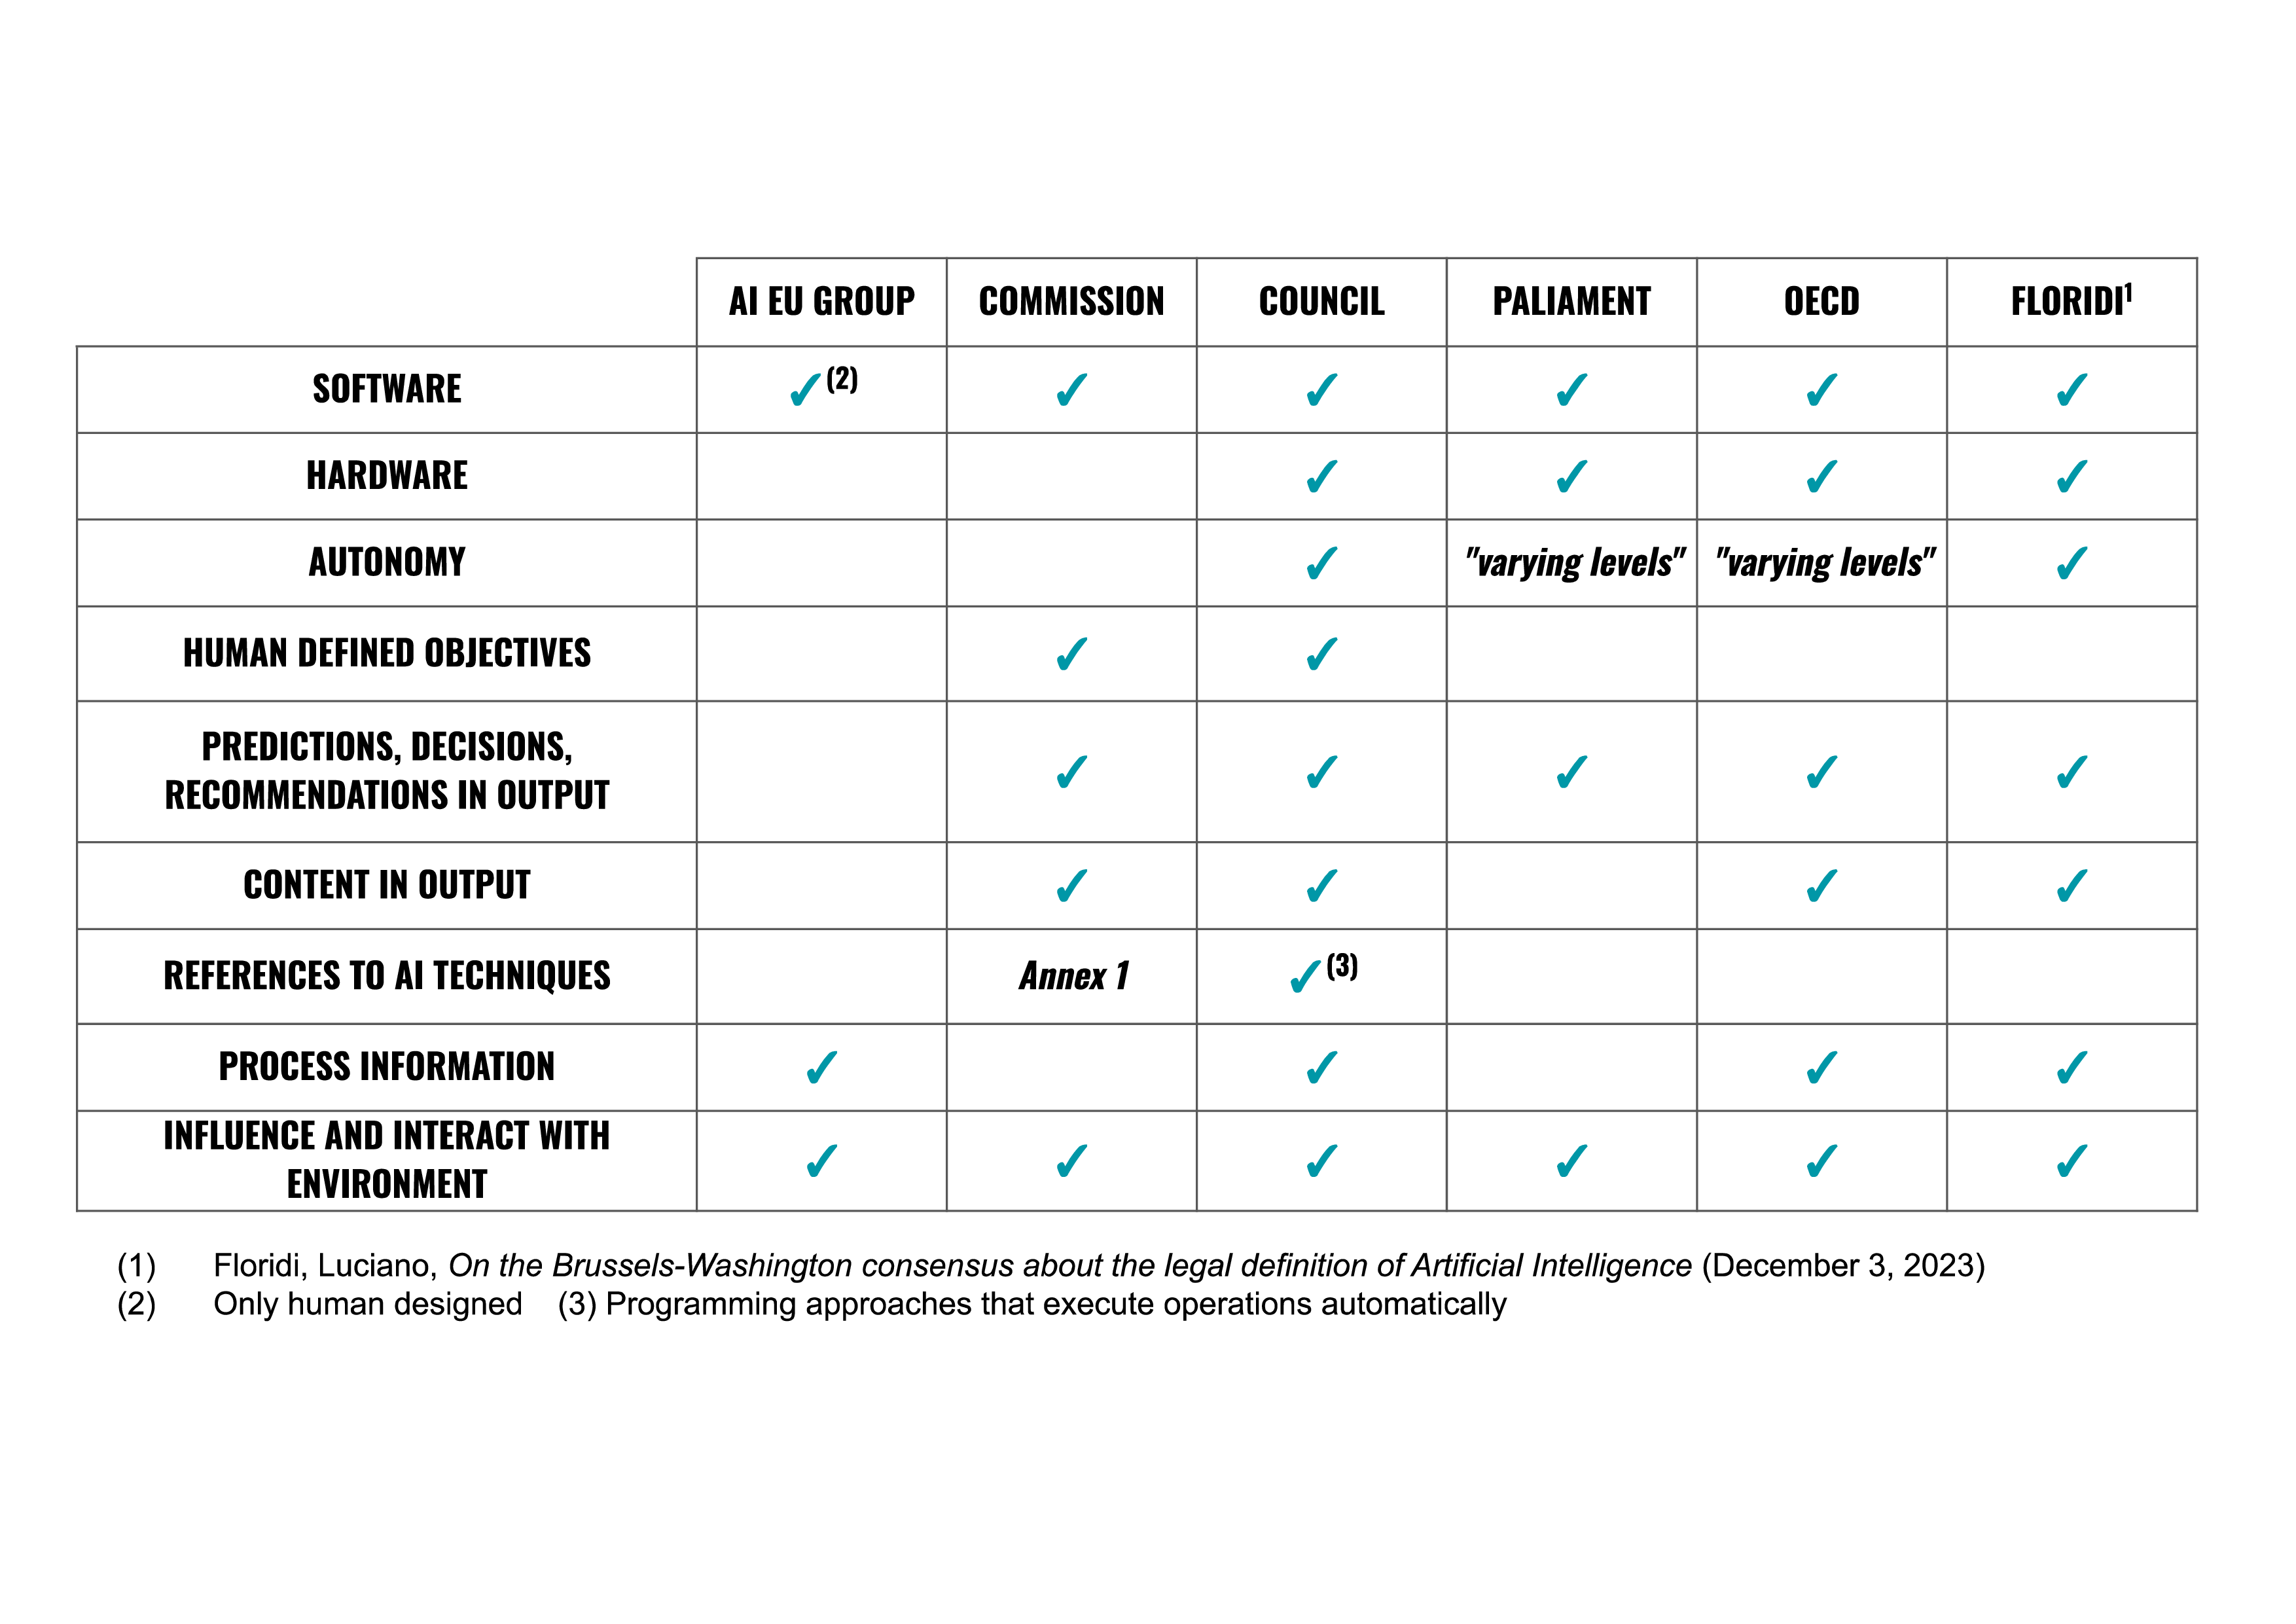
\includegraphics[width=1\linewidth]{img/image-001.png}
    \end{figure}
\end{frame}

\begin{frame}{Definitions applied to real cases}
    \begin{figure}
    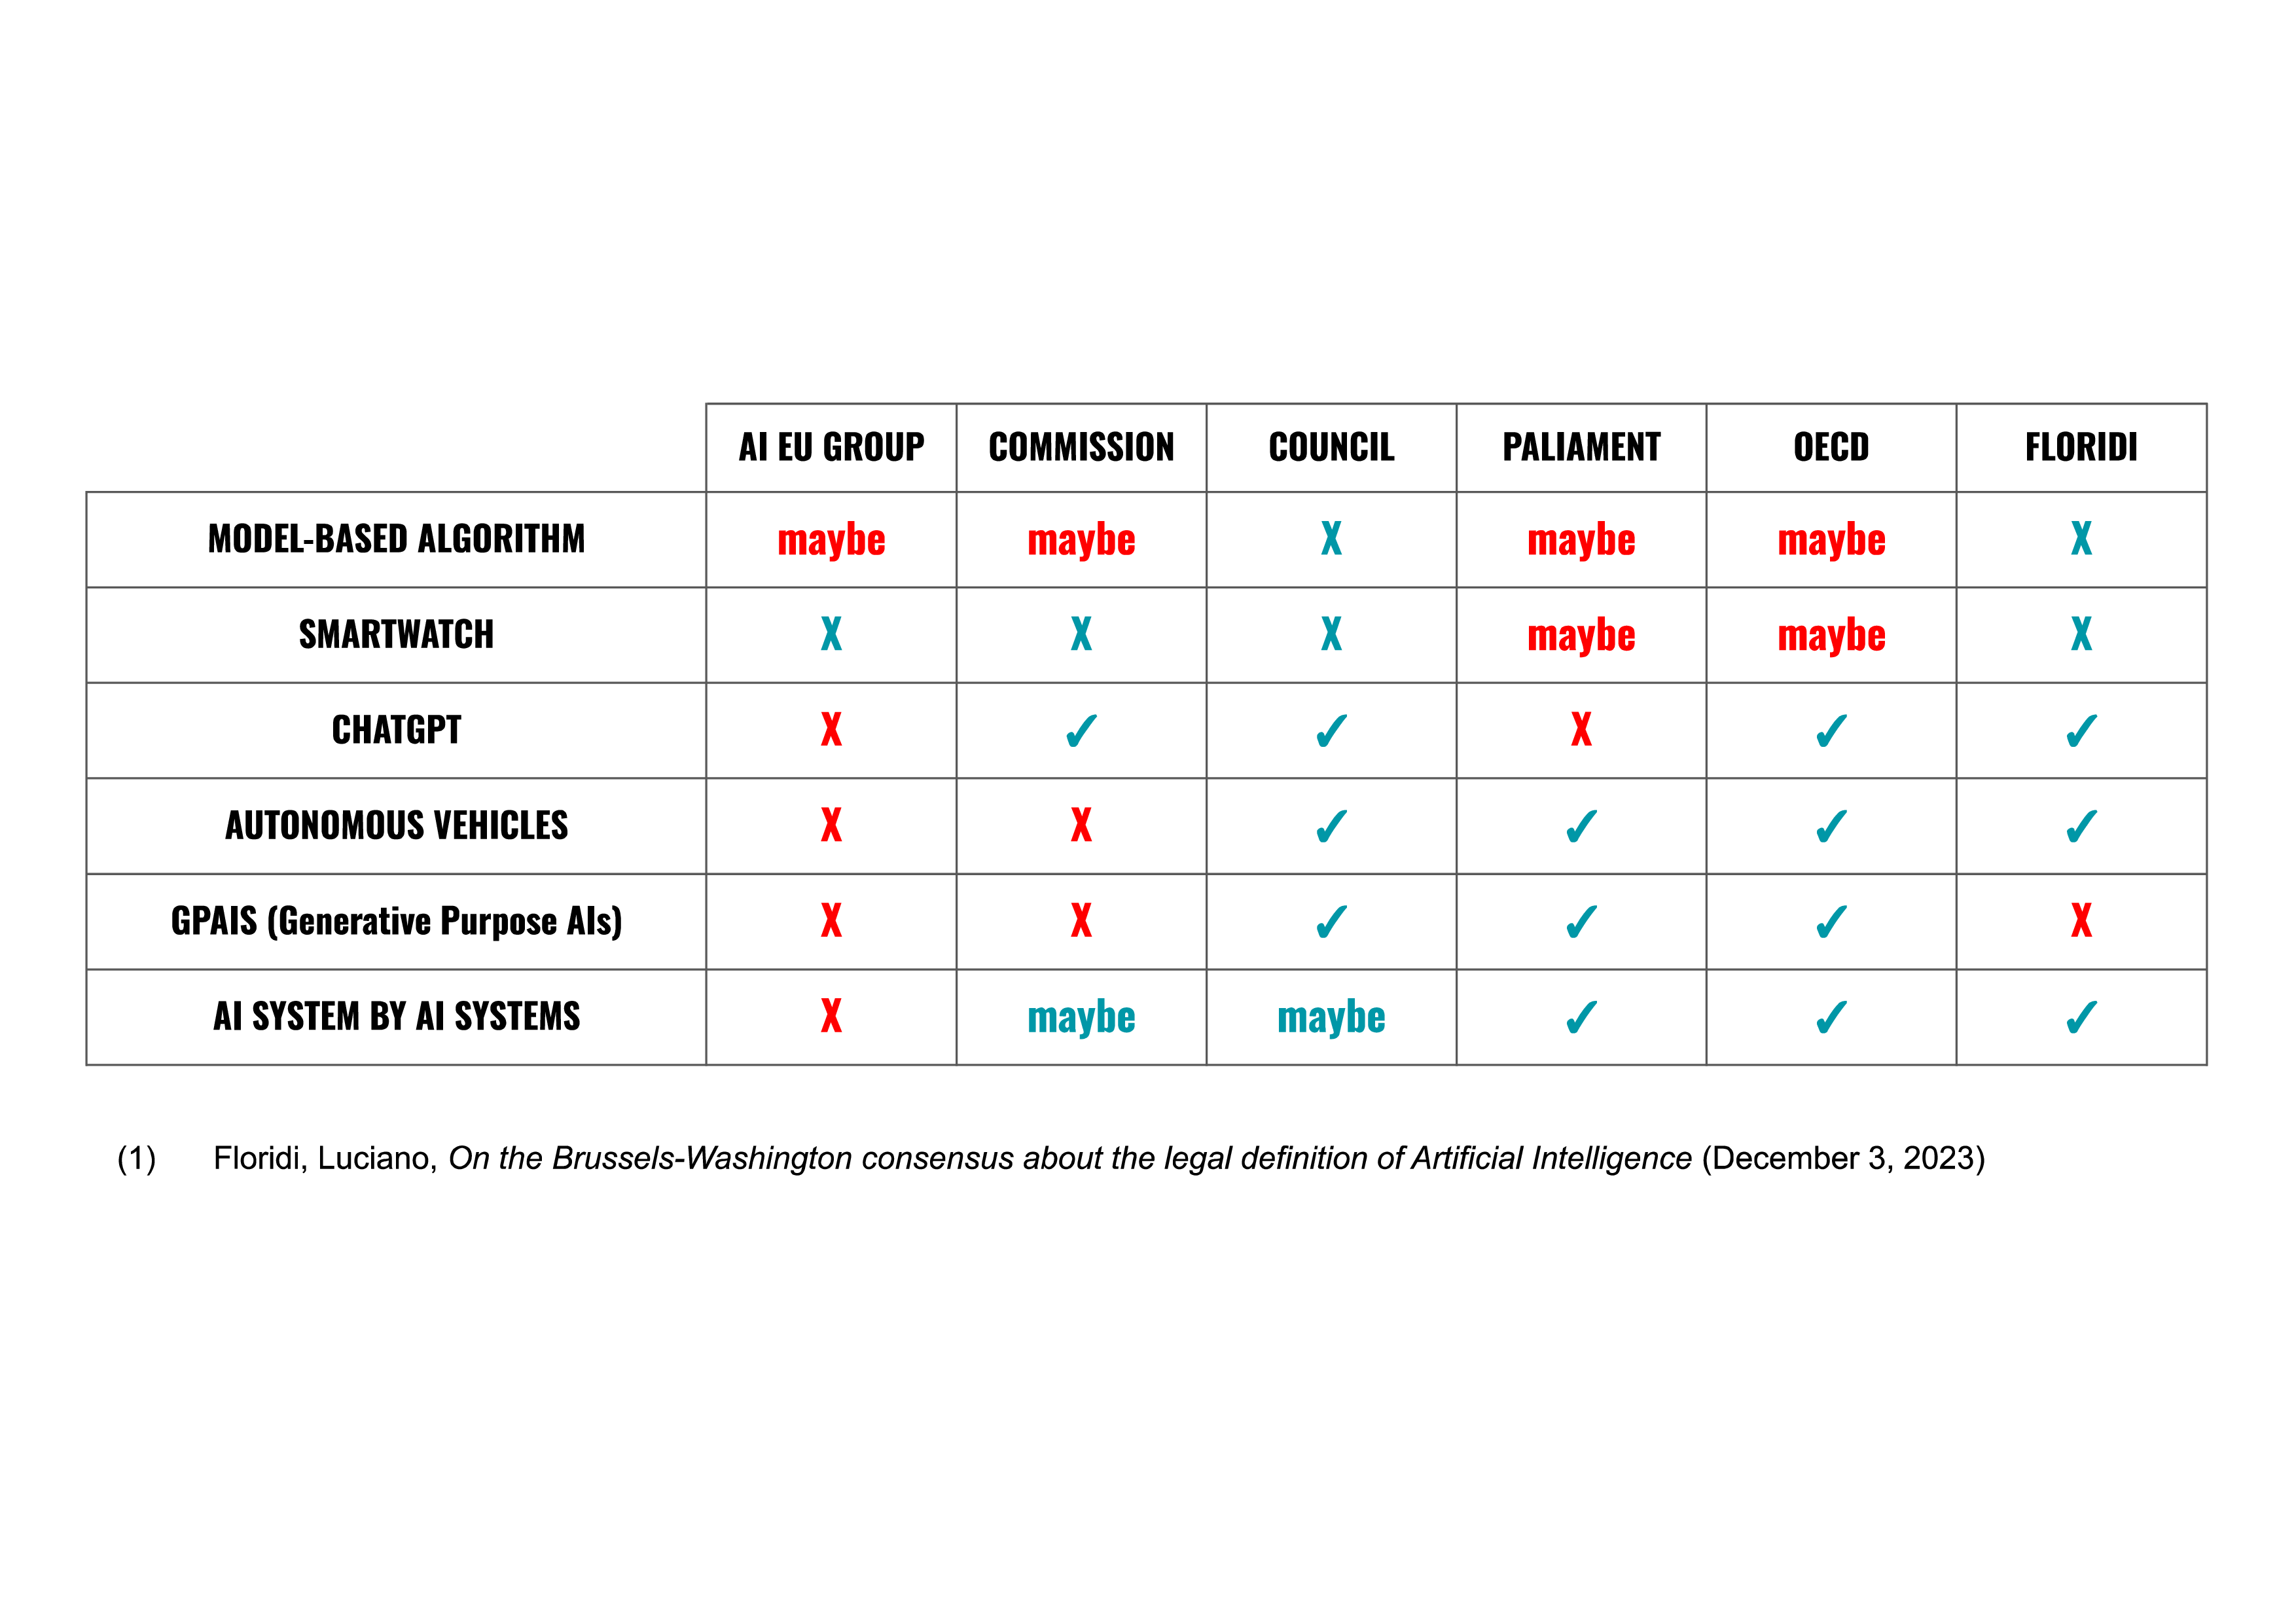
\includegraphics[width=1\linewidth]{img/image-002.png}
    \end{figure}
\end{frame}

\begin{frame}{Which is the best?}
\vfill
    \begin{quote}
    “Artificial Intelligence (AI) refers to an engineered system that can, for a given set of human-defined objectives, generate outputs – such as content, predictions, recommendations, or decisions – learn from historical data, improve its own behaviour, and influence people and environments”
    \end{quote}
    \vfill
    \begin{flushright}
    - Luciano Floridi\footnote{Floridi, Luciano, \emph{On the Brussels-Washington consensus about the legal definition of Artificial Intelligence} (December 3, 2023)}
  \end{flushright}
    
\end{frame}



\begin{frame}
\frametitle{Why is the best?}
\vspace{1.5em}
\begin{itemize}
\item \textcolor{teal}{\textbf{Great definition of “intelligence”}} : \textit{learn from historical data, improve its own behaviour, and influence people and environments}
\item \textcolor{teal}{\textbf{Transformative}} and “\textcolor{teal}{\textbf{Autonomy}}” properties included
\item Neither too broad, nor too specific
\item Includes what we consider AI technologies, leaving out those that aren't for us
\end{itemize}

\vspace{3.1em} % Adjust vertical space
\tiny
\begin{block}{}
\begin{quote}
    “Artificial Intelligence (AI) refers to an engineered system that can, for a given set of human-defined objectives, generate outputs – such as content, predictions, recommendations, or decisions – learn from historical data, improve its own behaviour, and influence people and environments”
    - Luciano Floridi\footnote[frame]{Floridi, Luciano, \emph{On the Brussels-Washington consensus about the legal definition of Artificial Intelligence} (December 3, 2023)}
\end{quote}\end{block}
\end{frame}

\begin{frame}
\frametitle{Possible issues?}
\vspace{1.5em}
\begin{itemize}
\item “Human-defined objectives” concept \textcolor{red}{\textbf{not really clear}}
    \bigskip
    \begin{itemize}
    \item can objectives also be defined by the machine itself?
    \begin{itemize}
        \item is “given a set of objectives \underline{\textbf{for}} human” better?
    \end{itemize}
    \bigskip
    \item “human-defined” means always human responsibility?
    \end{itemize}
    \bigskip
\item \textcolor{red}{\textbf{No}} references to any AI techniques or approach
    \begin{itemize}
        \item do we need it?
    \end{itemize}
    
\end{itemize}

\vspace{0.9em} % Adjust vertical space
\tiny
\begin{block}{}
\begin{quote}
    “Artificial Intelligence (AI) refers to an engineered system that can, for a given set of human-defined objectives, generate outputs – such as content, predictions, recommendations, or decisions – learn from historical data, improve its own behaviour, and influence people and environments”
    - Luciano Floridi\footnote[frame]{Floridi, Luciano, \emph{On the Brussels-Washington consensus about the legal definition of Artificial Intelligence} (December 3, 2023)}
\end{quote}\end{block}
\end{frame}

% \begin{frame}
% \frametitle{Multiple Columns}
% \begin{columns}[c] % The "c" option specifies centered vertical alignment while the "t" option is used for top vertical alignment

% \column{.45\textwidth} % Left column and width
% \textbf{Heading}
% \begin{enumerate}
% \item Statement
% \item Explanation
% \item Example
% \end{enumerate}

% \column{.5\textwidth} % Right column and width
% Lorem ipsum dolor sit amet, consectetur adipiscing elit. Integer lectus nisl, ultricies in feugiat rutrum, porttitor sit amet augue. Aliquam ut tortor mauris. Sed volutpat ante purus, quis accumsan dolor.

% \end{columns}
% \end{frame}

% %------------------------------------------------
% \section{Second Section}
% %------------------------------------------------

% \begin{frame}
% \frametitle{Table}
% \begin{table}
% \resizebox{\textwidth}{!}{%
% \begin{tabular}{p{5cm} c c c c c c}
% \textbf{} & \textbf{EU GROUP ON AI} & \textbf{COMMISSION} & \textbf{COUNCIL} & \textbf{PARLIAMENT} & \textbf{FLORIDI} & \textbf{OECD}\\
% \midrule
% SOFTWARE & $x$ (1) & $x$ & $x$ & $x$ & $x$ & $x$ \\
% HARDWARE & & & $x$ & $x$ & $x$ & $x$ \\
% AUTONOMY & & \textit{various levels} & $x$ & \textit{various levels} & $x$ & \textit{various levels} \\
% HUMAN DEFINED\\OBJECTIVES & & $x$ & $x$ & & $x$ & \\
% PREDICTIONS, RECOMMENDATIONS, OR DECISIONS IN OUTPUT & & $x$ & $x$ & $x$ & $x$ & $x$ \\
% CONTENT IN OUTPUT & & $x$ & $x$ & & $x$ & $x$ \\
% REFERNCES TO AI TECHNIQUES & & Annex 1 & $x$ (2) & & & \\
% PROCESS INFORMATION & $x$ & & $x$ & & $x$ & $x$ \\
% INFLUENCE AND INTERACT WITH ENVIRONMENT & $x$ & $x$ & $x$ & $x$ & $x$ & $x$ \\
% \end{tabular}%
% }
% \caption{Table caption}
% \end{table}
% \end{frame}
% \begin{frame}

% \begin{table}
%     \centering
%     \resizebox{\textwidth}{!}{
%     \begin{tabular}{|p{4 cm}|c|c|c|c|c|c|} \hline 
%          &   AI EU GROUP
% &   COMMISSION
% &   COUNCIL
% &   PARLIAMENT
% &  OECD
%  & FLORIDI1
% \\ \hline 
%           SOFTWARE
% &  ✓(2)
% &  ✓
% &  ✓
% &  ✓
% & ✓
%  &✓
% \\ \hline 
%          HARDWARE
% &   
% &   
% &  ✓
% &  ✓
% & ✓
%  &✓
% \\ \hline 
%          AUTONOMY
% &   
% &   
% &  ✓
% &  “varying levels”
% & “varying levels”
%  &✓
% \\ \hline 
%          HUMAN DEFINED \mbox{OBJECTIVES}
% &   
% &  ✓
% &  ✓
% &   
% &  
%  & 
% \\ \hline 
%          PREDICTIONS, DECISIONS, \mbox{RECOMMENDATIONS} IN OUTPUT
% &   
% &  ✓
% &  ✓
% &  ✓
% & ✓
%  &✓
% \\ \hline 
%          CONTENT IN OUTPUT
% &   
% &  ✓
% &  ✓
% &   
% & ✓
%  &✓
% \\ \hline 
%          REFERENCES TO AI TECHNIQUES
% &   
% &  Annex 1
% &  ✓(3)
% &   
% &  
%  & 
% \\ \hline 
%          PROCESS INFORMATION
% &  ✓
% &   
% &  ✓
% &   
% & ✓
%  &✓
% \\ \hline
%     \end{tabular}
%     }
%     \caption{Caption 1}
%     \label{tab:t1}
% \end{table}
% \end{frame}


% \begin{frame}
% % Please add the following required packages to your document preamble:
% % \usepackage{graphicx}
% % \usepackage[table,xcdraw]{xcolor}
% % Beamer presentation requires \usepackage{colortbl} instead of \usepackage[table,xcdraw]{xcolor}
% \begin{table}[]
% \resizebox{\textwidth}{!}{%
% \begin{tabular}{|p{5cm}|p{2cm}|p{2cm}|p{2cm}|p{2cm}|p{2cm}|p{2cm}|}
% \hline
% \textbf{} &
%   \multicolumn{1}{c|}{\textbf{AI EU GROUP}} &
%   \textbf{COMMISSION} &
%   \textbf{COUNCIL} &
%   \textbf{PALIAMENT} &
%   \textbf{OECD} &
%   \textbf{FLORIDI1} \\ \hline
% \textbf{SOFTWARE} &
%   \multicolumn{1}{c|}{{\color[HTML]{32CB00} \textbf{✓(2)}}} &
%   {\color[HTML]{32CB00} \textbf{✓}} &
%   {\color[HTML]{32CB00} \textbf{✓}} &
%   {\color[HTML]{32CB00} \textbf{✓}} &
%   {\color[HTML]{32CB00} \textbf{✓}} &
%   {\color[HTML]{32CB00} \textbf{✓}} \\ \hline
% \textbf{HARDWARE} &
%    &
%   \multicolumn{1}{l|}{} &
%   {\color[HTML]{32CB00} \textbf{✓}} &
%   {\color[HTML]{32CB00} \textbf{✓}} &
%   {\color[HTML]{32CB00} \textbf{✓}} &
%   {\color[HTML]{32CB00} \textbf{✓}} \\ \hline
% \textbf{AUTONOMY} &
%    &
%   \multicolumn{1}{l|}{} &
%   {\color[HTML]{32CB00} \textbf{✓}} &
%   \textit{\textbf{"varying levels"}} &
%   \textit{\textbf{"varying levels"}} &
%   {\color[HTML]{0097A7} \textbf{✓}} \\ \hline
% \textbf{HUMAN DEFINED OBJECTIVES} &
%    &
%   {\color[HTML]{32CB00} \textbf{✓}} &
%   {\color[HTML]{32CB00} \textbf{✓}} &
%   \multicolumn{1}{l|}{} &
%   \multicolumn{1}{l|}{} &
%   \multicolumn{1}{l|}{} \\ \hline
% \textbf{PREDICTIONS, DECISIONS, RECOMMENDATIONS IN OUTPUT} &
%    &
%   {\color[HTML]{32CB00} \textbf{✓}} &
%   {\color[HTML]{32CB00} \textbf{✓}} &
%   {\color[HTML]{32CB00} \textbf{✓}} &
%   {\color[HTML]{32CB00} \textbf{✓}} &
%   {\color[HTML]{32CB00} \textbf{✓}} \\ \hline
% \textbf{CONTENT IN OUTPUT} &
%    &
%   {\color[HTML]{32CB00} \textbf{✓}} &
%   {\color[HTML]{32CB00} \textbf{✓}} &
%   \multicolumn{1}{l|}{} &
%   {\color[HTML]{32CB00} \textbf{✓}} &
%   {\color[HTML]{32CB00} \textbf{✓}} \\ \hline
% \textbf{REFERENCES TO AI TECHNIQUES} &
%    &
%   \textit{\textbf{Annex 1}} &
%   {\color[HTML]{32CB00} \textbf{✓(3)}} &
%   \multicolumn{1}{l|}{} &
%   \multicolumn{1}{l|}{} &
%   \multicolumn{1}{l|}{} \\ \hline
% \textbf{PROCESS INFORMATION} &
%   \multicolumn{1}{c|}{{\color[HTML]{32CB00} \textbf{✓}}} &
%   \multicolumn{1}{l|}{} &
%   {\color[HTML]{32CB00} \textbf{✓}} &
%   \multicolumn{1}{l|}{} &
%   {\color[HTML]{32CB00} \textbf{✓}} &
%   {\color[HTML]{32CB00} \textbf{✓}} \\ \hline
% \textbf{INFLUENCE AND INTERACT WITH ENVIRONMENT} &
%   \multicolumn{1}{c|}{{\color[HTML]{32CB00} \textbf{✓}}} &
%   {\color[HTML]{32CB00} \textbf{✓}} &
%   {\color[HTML]{32CB00} \textbf{✓}} &
%   {\color[HTML]{32CB00} \textbf{✓}} &
%   {\color[HTML]{32CB00} \textbf{✓}} &
%   {\color[HTML]{32CB00} \textbf{✓}} \\ \hline
% \end{tabular}%
% }
% \end{table}
% \end{frame}


% %------------------------------------------------

% \begin{frame}
% \frametitle{Theorem}
% \begin{theorem}[Mass--energy equivalence]
% $E = mc^2$
% \end{theorem}
% \end{frame}

% %------------------------------------------------

% \begin{frame}[fragile] % Need to use the fragile option when verbatim is used in the slide
% \frametitle{Verbatim}
% \begin{example}[Theorem Slide Code]
% \begin{verbatim}
% \begin{frame}
% \frametitle{Theorem}
% \begin{theorem}[Mass--energy equivalence]
% $E = mc^2$
% \end{theorem}
% \end{frame}\end{verbatim}
% \end{example}
% \end{frame}

% %------------------------------------------------

% \begin{frame}
% \frametitle{Figure}
% Uncomment the code on this slide to include your own image from the same directory as the template .TeX file.
% %\begin{figure}
% %\includegraphics[width=0.8\linewidth]{test}
% %\end{figure}
% \end{frame}

% %------------------------------------------------

% \begin{frame}[fragile] % Need to use the fragile option when verbatim is used in the slide
% \frametitle{Citation}
% An example of the \verb|\cite| command to cite within the presentation:\\~

% This statement requires citation \cite{p1}.
% \end{frame}

% %------------------------------------------------

% \begin{frame}
% \frametitle{References}
% \footnotesize{
% \begin{thebibliography}{99} % Beamer does not support BibTeX so references must be inserted manually as below
% \bibitem[Smith, 2012]{p1} John Smith (2012)
% \newblock Title of the publication
% \newblock \emph{Journal Name} 12(3), 45 -- 678.
% \end{thebibliography}
% }
% \end{frame}

% %------------------------------------------------


\begin{frame}
\Huge{\centerline{Thanks for the attention}}
\end{frame}

%----------------------------------------------------------------------------------------

\begin{frame}[noframenumbering]
\frametitle{Appendix 1}
\begin{block}{EU Expert Group on AI}
‘artificial intelligence system’ (AI system) means software systems designed by humans that, given a complex goal, act in the physical or digital dimension by perceiving their environment through data acquisition, interpreting the collected structured or unstructured data, reasoning on the knowledge, or processing the information, derived from this data and deciding the best action(s) to take to achieve the given goal.
\end{block}

\begin{block}{Commission}
‘artificial intelligence system’ (AI system) means software that is developed with one or more of the techniques and approaches listed in Annex I and can, for a given set of human-defined objectives, generate outputs such as content, predictions, recommendations, or decisions influencing the environments they interact with.
\end{block}
\end{frame}
\begin{frame}[noframenumbering]
\frametitle{Appendix 2}
\begin{block}{Council}
‘artificial intelligence system’ (AI system) means a system that is designed to operate with elements of autonomy and that, based on machine and/or human provided data and inputs, infers how to achieve a given set of objectives using machine learning and/or logic- and knowledge based approaches, and produces system-generated outputs such as content (generative AI systems), predictions, recommendations or decisions, influencing the environments with which the AI system interacts.
\end{block}

\begin{block}{Parliament}
’artificial intelligence system’ (AI system) means a machine-based system that is designed to operate with varying levels of autonomy and that can, for explicit or implicit objectives, generate outputs such as predictions, recommendations, or decisions, that influence physical or virtual environments.
\end{block}
\end{frame}
\begin{frame}[noframenumbering]
\frametitle{Appendix 3}
\begin{block}{OECD.AI}
An AI system is a machine-based system that, for explicit or implicit objectives, infers, from the input it receives, how to generate outputs such as predictions, content, recommendations, or decisions that can influence physical or virtual environments. Different AI systems vary in their levels of autonomy and adaptiveness after deployment.
\end{block}
\begin{block}{Luciano Floridi\footnote[frame]{Floridi, Luciano, \emph{On the Brussels-Washington consensus about the legal definition of Artificial Intelligence} (December 3, 2023)}}
Artificial Intelligence (AI) refers to an engineered system that can, for a given set of human-defined objectives, generate outputs – such as content, predictions, recommendations, or decisions – learn from historical data, improve its own behaviour, and influence people and environments.
\end{block}

\end{frame}

\end{document}